\section{ArrayList}
\subsection{Definitie}
\begin{frame}{\dsarraylist{}: definitie}
\begin{definition}[\dsarraylist{}]
Een \term{\dsarraylist{}} is een gegevensstructuur die bestaat uit een opeenvolging van elementen. Elk element in een \dsarraylist{} heeft een unieke \term{index} en is toegankelijk in constante tijd (dit wordt ook wel \term{Random-Access} genoemd). Een \dsarraylist{} heeft een variabele \term{lengte}: we hoeven geen lengte op te geven bij de constructie van een \dsarraylist{} en in principe kunnen we eindeloos elementen toevoegen.
\end{definition}
Visueel zullen we een \dsarraylist{} in deze presentatie voorstellen als een opeenvolging van hokjes, maar met een open einde. Zoals hier:
\begin{figure}
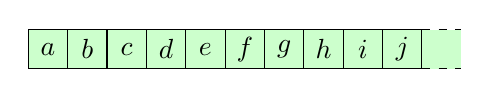
\begin{tikzpicture}
\fill[fill=green!20] (0,0) rectangle (5.5,0.5);
\draw (0,0) rectangle (5,0.5);
\draw[dashed] (5,0) -- ++(0.5,0);
\draw[dashed] (5,0.5) -- ++(0.5,0);
\foreach \x in {1,2,...,9} {
  \draw (0.5*\x,0) -- ++(0,0.5);
}
\foreach \x/\t in {0/a,1/b,2/c,3/d,4/e,5/f,6/g,7/h,8/i,9/j} {
  \draw (0.5*\x+0.25,0.25) node {$\t$};
}
\end{tikzpicture}
\caption{Voorstelling van een \dsarraylist{}}
\end{figure}
\end{frame}
\subsection{In Java}
\subsubsection{Declaratie}
\begin{frame}[fragile]{\dsarraylist{} in Java: declaratie}
Een \dsarraylist{} is een klasse die uit de Java-bibliotheek komt. Deze klasse is \texttt{java.util.ArrayList}. Daarom kunnen we een \dsarraylist{} aanmaken zoals andere objecten. Een \dsarraylist{} is een \term{generische klasse}: we kunnen een type-parameter tussen scheve haken (\texttt{<>}).
\begin{example}[Declaratie \dsarraylist{}]
\begin{lstlisting}
import java.util.ArrayList;

ArrayList<Integer> lijstMetGetallen = new ArrayList<Integer>();

ArrayList<Paard> lijstMetPaarden = new ArrayList<Paard>();

ArrayList<ArrayList<Integer>> lijstMetLijstenMetGetallen =
    new ArrayList<ArrayList<Integer>>();
\end{lstlisting}
\end{example}
\end{frame}
\begin{frame}[fragile]{\dsarraylist{} in Java: Primitieve types bij generische klasses}
\begin{letop}[Primitieve types bij generische klasses]
\small{Men kan een \dsarraylist{} declareren met elk \term{klasse-type}, primitieve types zijn niet toegelaten! Hiervoor heeft Java schaduwklasses ingevoerd:}
\begin{table}
\centering
\small{\begin{tabular}{l|l}
Primitief type&Klasse-type\\\hline
\texttt{byte}&\texttt{Byte}\\
\texttt{short}&\texttt{Short}\\
\texttt{int}&\texttt{Integer}\\
\texttt{long}&\texttt{Long}\\
\texttt{float}&\texttt{Float}\\
\texttt{double}&\texttt{Double}\\
\texttt{boolean}&\texttt{Boolean}\\
\texttt{char}&\texttt{Char}\\
\end{tabular}}
\caption{Omzetten van primitieve types naar klasse-types}
\end{table}
\end{letop}
\end{frame}
\subsubsection{Toevoegen en verwijderen}
\begin{frame}[fragile]{\dsarraylist{} in Java: toevoegen/verwijderen van elementen}
\dsarraylist{} biedt methodes aan om elementen toe te voegen en te verwijderen:
\small{\begin{itemize}
 \item \texttt{public boolean add (E element)}: voegt een element toe op het einde van de \dsarraylist{}
 \item \texttt{public void add (int index, E element)}: voegt een element toe op plaats \texttt{index}, de overige elementen worden naar rechts opgeschoven
 \item \texttt{public E remove (int index)}: verwijdert het element op \texttt{index}. De elementen erna worden naar links opgeschoven. Het element die oorspronkelijk op deze plaats stond, wordt teruggegeven
 \item \texttt{public boolean remove (Object o)}: het opgegeven element wordt uit de \dsarraylist{} verwijdert. Geeft \texttt{true} terug indien dit element in de \dsarraylist{} aanwezig was.
\end{itemize}}
\end{frame}
\begin{frame}[fragile]{\dsarraylist{} in Java: \texttt{add (E element)}}
\begin{methodexample}
\begin{center}
\begin{animateinline}[poster=first,controls]{1}
\methodexec{arraylistadd0me.java}{1}
\end{animateinline}
\end{center}
\end{methodexample}
\end{frame}
\begin{frame}[fragile]{\dsarraylist{} in Java: \texttt{add (int index, E element)}}
\begin{methodexample}

\end{methodexample}
\end{frame}
\begin{frame}[fragile]{\dsarraylist{} in Java: \texttt{remove (int index)}}
\begin{methodexample}

\end{methodexample}
\end{frame}
\begin{frame}[fragile]{\dsarraylist{} in Java: \texttt{remove (Object o)}}
\begin{methodexample}

\end{methodexample}
\end{frame}
\subsubsection{Toegang tot elementen}
\begin{frame}[fragile]{\dsarraylist{} in Java: toegang tot elementen}
Omdat \dsarraylist{} een gewone klasse is, krijgt met toegang tot de elementen via methodes:
\begin{itemize}
 \item \texttt{public E get (int index)}
 \item \texttt{public E set (int index, E element)}
\end{itemize}
\end{frame}
\subsection{Lengte}
\begin{frame}[fragile]{\dsarraylist{} in Java: lengte (aantal elementen)}
We kunnen het aantal elementen in de \dsarraylist{} opvragen met behulp van de \texttt{size()}-methode.
\begin{example}[Lengte van een \dsarraylist{}]
\begin{lstlisting}
ArrayList<String> namen = new ArrayList<String>();
namen.add("Samson");
namen.add("Gert");
namen.add("Alberto");
namen.add("Octaaf");
System.out.println(namen.size()); //4
\end{lstlisting}
\end{example}
\begin{letop}[\texttt{length} versus \texttt{size()}]
Bij een \dsarray{} vragen we de lengte op met behulp van \texttt{.length}. Bij een \dsarraylist{} is dat met de \texttt{size()}-methode. Omgekeerd werkt dit niet!
\end{letop}
\end{frame}
\subsubsection{Andere operaties}
\subsection{Werking}
\subsection{Implementatie}